\subsection{\texorpdfstring{CLOSED SUBGROUPS OF \(\mathbf{R}^n\)}{CLOSED SUBGROUPS OF R TO THE N}}

We know already of two types of closed subgroups of \(\mathbf{R}^n\) ; on the one hand, the vector subspaces of \(\mathbf{R}^n\) , which are isomorphic to the groups \(\mathbf{R}^p\) ( \(p \leqslant n\) ) (Chapter IV, § 1, no. 4, Proposition 2); on the other hand, the discrete subgroups (Chapter III, § 2, no. 1, Proposition 5) which are isomorphic to groups \(\mathbf{Z}^q\) ( \(q \leqslant n\) ), as we have just seen. We shall now determine the structure of an arbitrary closed subgroup of \(\mathbf{R}^n\) by showing that such a subgroup is isomorphic to a product of the form

\[
\mathbf {R} ^ {p} \times \mathbf {Z} ^ {q} \quad \text { where } \quad \mathrm{o} \leqslant p + q \leqslant n.
\]

The proof rests on the following proposition:

PROPOSITION 3. Every non-discrete closed subgroup of \(\mathbf{R}^n\) contains a line passing through o.

Let \((\pmb{x}_p)_{p\in \mathbb{N}}\) be an infinite sequence of points of \(\mathbf{G}\) such that \(\pmb{x}_p\neq 0\) and \(\lim_{p\to \infty}\pmb{x}_p = 0\) ; by hypothesis such a sequence exists. Let \(\mathbf{P}\) be an open cube with centre \(0\) , containing the \(\pmb{x}_p\) . Let \(k_{p}\) denote the largest integer \(h > 0\) such that \(h\pmb{x}_p\in \mathrm{P}\) (since \(\mathbf{P}\) is a bounded box and \(\pmb{x}_p\neq 0\) , the existence of \(k_{p}\) follows from Archimedes' axiom). The points \(k_{p}\pmb{x}_{p}\) lie in a compact set \(\overline{\mathrm{P}}\) , hence the sequence \((k_{p}\pmb{x}_{p})_{p\in \mathbb{N}}\) has a cluster point \(\pmb {a}\in \overline{\mathrm{P}}\) . If \(||k_p\pmb {x}_p - \pmb {a}||\leqslant \varepsilon\) , we have

\[
\left| \left| \left(k _ {p} + \mathrm{I}\right) x _ {p} - a \right| \right| \leqslant \varepsilon + \left| \left| x _ {p} \right| \right|,
\]

and since \(\lim_{p\to \infty}\boldsymbol{x}_p = 0\) , it follows that \(\boldsymbol{a}\) is also a cluster point of the sequence \(((k_p + 1)x_p)\) , whose points belong to the closed set \(\mathfrak{C}P\) , by definition of \(k_{p}\) ; hence \(\boldsymbol{a} \in \overline{\mathrm{P}} \cap \mathfrak{C}P\) (the frontier of P, Fig. 5), which implies \(\boldsymbol{a} \neq 0\) . Moreover, since G is closed, we have \(\boldsymbol{a} \in \mathrm{G}\) . Let \(t\) be any real number; since \(|tk_p - [tk_p]| < 1\) , the relation \(||k_p x_p - a|| \leqslant \varepsilon\) implies that \(||[tk_p]x_p - ta|| \leqslant |t| \varepsilon + ||x_p||\) ; since \(\lim_{p \to \infty} x_p = 0\) , \(ta\) is a

\pandocbounded{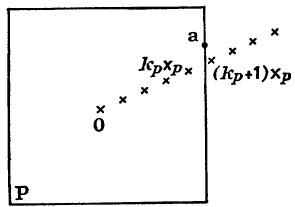
\includegraphics[keepaspectratio]{images/part001_2a0a1c84.jpg}}\\
Figure 5.

\pandocbounded{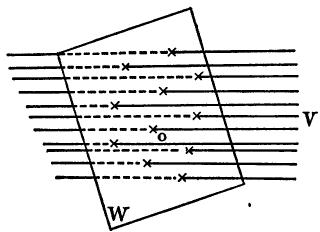
\includegraphics[keepaspectratio]{images/part001_3dc381fa.jpg}}\\
Figure 6.

cluster point of the sequence \(([tk_p]x_p)\) ; but the points of this sequence belong to G, and consequently \(ta \in G\) , since G is closed. This completes the proof.

THEOREM 2. Let G be a closed subgroup of \(\mathbf{R}^n\) , of rank \(r\) ( \(0 \leqslant r \leqslant n\) ). Then there is a largest vector subspace V contained in G; for every vector subspace W complementary to V, W ∩ G is discrete and G is the direct sum of V and W ∩ G.

Let us first establish the existence of V by showing that the union of all the lines through o which lie in G is a vector subspace: indeed, the vector subspace generated by the union of these lines is the same as the subgroup they generate. The group G is the direct sum of V and W ∩ G; for if \(x \in G\) , we have \(x = y + z\) where \(y \in V\) and \(z \in W\) ; since \(V \subset G\) , \(z = x - y \in G\) and therefore \(z \in W \cap G\) . It remains to show that \(W \cap G\) is discrete; this follows from Proposition 3, since \(W \cap G\) is a closed subgroup which contains no lines, by reason of the definition of V.

If \(G \neq V\) , we may say that G is the union of a countable infinity of linear varieties, parallel to V and passing through the points of the discrete group \(W \cap G\) (Fig. 6).

If \(p\) is the dimension of the vector subspace \(\mathbf{V}\) , we have \(p \leqslant r\) , and \(\mathbf{W} \cap \mathbf{G}\) is a discrete group of rank \(r - p\) .

COROLLARY 1. There exists a basis \((\pmb{a}_i)_{1\leqslant i\leqslant n}\) of \(\mathbf{R}^n\) , such that

\[
\boldsymbol {a} _ {i} \in \mathrm{G} \quad (\mathrm{I} \leqslant i \leqslant r), \quad \boldsymbol {a} _ {i} \in \mathrm{V} \quad (\mathrm{I} \leqslant i \leqslant p)
\]

and such that \(\mathbf{G}\) is the set of points \(\sum_{i=1}^{p} t_i a_i + \sum_{j=p+1}^{r} n_j a_j\) , where the \(t_i\) take all real values and the \(n_j\) take all integer values.

This follows from Theorem 2, and Theorem 1 of no. 1 applied to the discrete group \(W \cap G\) .

COROLLARY 2. There exists an automorphism of \(\mathbf{R}^n\) which maps \(\mathbf{G}\) onto the group \(\mathbf{G}'\) , isomorphic to \(\mathbf{R}^p \times \mathbf{Z}^{r-p}\) , which is the direct sum of the vector subspace generated by \(e_1, e_2, \ldots, e_p\) and the (discrete) additive subgroup generated by \(e_{p+1}, e_{p+2}, \ldots, e_r\) .

This is an immediate consequence of Corollary 1. Corollary 2 of Theorem 2 shows that a closed subgroup G of \(R^{n}\) is completely determined up to isomorphism by two integers \(\geqslant 0\) : its rank, which we denote by \(r(\mathbf{G})\) , and the dimension of the largest vector subspace contained in G, which we call the dimension of G and denote by \(d(\mathbf{G})\) .

The only conditions which these integers have to satisfy are the inequalities \(o \leqslant d(\mathbf{G}) \leqslant r(\mathbf{G}) \leqslant n\) .

